\documentclass[a4paper, 10pt]{article}
%\usepackage[utf8]{inputenc}			
\usepackage[german]{babel}		% for german	
\usepackage[dvips]{graphicx}		
\usepackage{psfrag}						
\usepackage{parskip}
\usepackage{listings}
\usepackage{xcolor}
\usepackage{amsmath}
\usepackage{mathtools}
\usepackage{amssymb}
\usepackage{mathrsfs}
\usepackage{empheq}
\usepackage{titlesec}	
\usepackage{tikz}
\usetikzlibrary{arrows, shapes}
\usepackage{epstopdf}
\usepackage{dsfont}
\usepackage{sectsty}
\allsectionsfont{\bfseries\sffamily}

\addtolength{\textwidth}{2.1cm}
\addtolength{\topmargin}{-1.4cm}
\addtolength{\oddsidemargin}{-1.1 cm}
\definecolor{leichtgrau}{gray}{0.91}
\setlength{\parindent}{0pt}

% \lstset{language = C,
	% basicstyle=\footnotesize,       
	% numbers=left,                  
	% numberstyle=\footnotesize,      
	% stepnumber=2,
	% numbersep=5pt,
	% backgroundcolor=\color{leichtgrau},
	% frame=single,
% }

% Definition von römischen Zahlen
\makeatletter
\newcommand{\rmnum}[1]{\romannumeral #1}
\newcommand{\Rmnum}[1]{\expandafter\@slowromancap\romannumeral #1@}
\makeatother
%\renewcommand{\familydefault}{\sfdefault}


\begin{document}
\setcounter{section}{2}
\tableofcontents
\section{Multiuser MIMO}
\begin{itemize}
	\item We distinguish two cases:
	\begin{itemize}
		\item multipoint\,-\,to\,-\,point transmission
		\item point\,-\,to\,-\,multipoint transmission
	\end{itemize}
	\item Multipoint\,-\,to\,-\,point transmission
	\begin{itemize}
		\item typical uplink scenario in cellular systems
		\item information theoretical channel model: Multiple Access Channel (MAC)
		\begin{figure}[h]\centering
			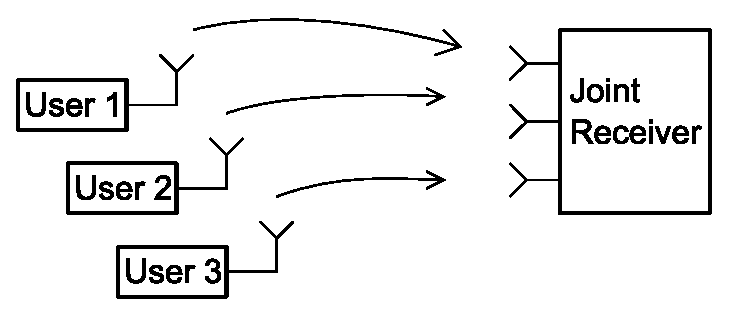
\includegraphics[scale=0.8]{MAC}
		\end{figure}
%		\begin{tikzpicture}
%			\node (user1) at (0,0) [draw] {User 1};
%			\node (user2) at (1,-1)[draw] {User 2};
%			\node (user3) at (2,-2)[draw] {User 3};		
%			\draw[-<] (user1.east) --(1,0) --(1,0.5);        
%			\draw[-<] (user2.east) --(2,-1) --(2,-0.5); 
%			\draw[-<] (user3.east) --(3,-2) --(3,-1.5); 
%			\node[draw, minimum width = 2cm, minimum height = 2.5cm, font = \bfseries\large] (Joint_Receiver) at (10,-1) {Joint Receiver};
%			\path[draw,-<] ([xshift = 0cm, yshift = 0.5cm] Joint_Receiver.west)--([xshift = -1cm, yshift = 0.5cm] Joint_Receiver.west);
%			\path[draw,-<] (Joint_Receiver.west)--([xshift = -1cm, yshift = 0cm] Joint_Receiver.west) ;
%			\path[draw,-<] ([xshift = 0cm, yshift = -0.5cm] Joint_Receiver.west)--([xshift = -1cm, yshift = -0.5cm] Joint_Receiver.west);
%			\path[draw,->,>=stealth'] ([xshift = 0.6cm,yshift = 0.4cm] user1.east)--([xshift = -2.5cm, yshift = 0.5cm] Joint_Receiver.west);
%			\path[draw,->,>=stealth'] ([xshift = 0.6cm,yshift = 0.4cm] user2.east)--([xshift = -2.5cm, yshift = 0cm] Joint_Receiver.west);
%			\path[draw,->,>=stealth'] ([xshift = 0.6cm,yshift = 0.4cm] user3.east)--([xshift = -2.5cm, yshift = -0.5cm] Joint_Receiver.west);
%		\end{tikzpicture}
	\end{itemize}
	\item Point\,-\,to\,-multipoint transmission
	\begin{itemize}
		\item typical downlink scenarion in cellular systems
		\item information theoretical channel model: Broadcast Channel (BC)
		\begin{figure}[h]\centering
			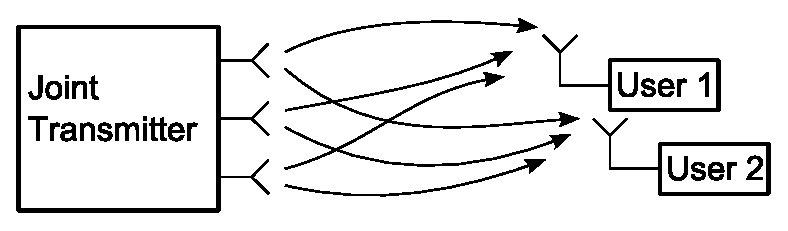
\includegraphics[scale=0.8]{BC}
		\end{figure}	
	\end{itemize}
	\item Advantage of multiuser MIMO compared to point\,-\,to\,-\,point MIMO
	\begin{itemize}
		\item multiplexing gain can be exploited even if users have only single antenna
		\item users are spatially distributed in cell $\rightarrow $ channels to different users are independent
	\end{itemize}
\end{itemize}
\subsection{Multiple Access Channel (MAC)}
We consider two aspects:
\begin{itemize}
	\item Detector structures
	\item Rate region
\end{itemize}
\subsubsection{Detector structures}
\paragraph*{Channel model:}
\begin{figure}[h]\centering
	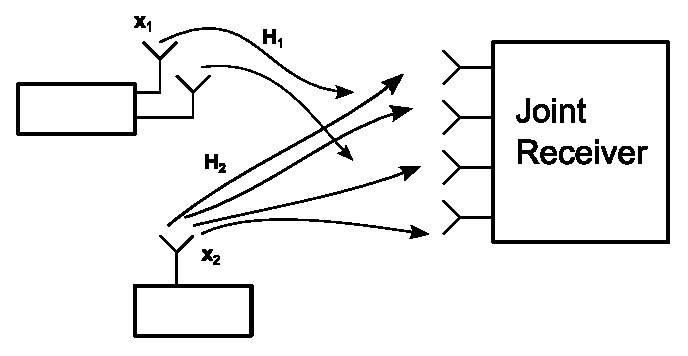
\includegraphics[scale=0.8]{Detector_Structures_Channel_Model}
\end{figure}
$\rightarrow  $ general MAC: $\mathbf{y} = \sum\limits_{k = 1}^{K}\mathbf{H}_k\mathbf{x}_k + \mathbf{n} $\\
with: \begin{itemize}
	\item K users
	\item user $k $ has $N_{T,k} $ transmit antennas
	\item $N_R $ receive antennas
	\item $\mathbf{H}_k \in \mathbb{C}^{N_R\times N_{T,k}} $ 
\end{itemize}
\begin{align*}
	\mathbf{y} = 
	\underbrace{
	\begin{bmatrix}\mathbf{H}_1 & \mathbf{H}_2 & \ldots & \mathbf{H}_k 	
	\end{bmatrix}
	}_{\mathbf{H}}\cdot
	\underbrace{
	\begin{bmatrix}\mathbf{x}_1 \\ \vdots \\ \mathbf{x}_k		
	\end{bmatrix}}_{\mathbf{x}} + \mathbf{n}
\end{align*}
\paragraph*{Observation:}
\begin{itemize}
	\item same equivalent channel model as for a point\,-\,to\,-\,point MIMO system transmitting $N_T = \sum_{k = 1}^{K} N_{T,k} $ independent signal streams \quad \textit{(Anmerkung: kein Unterschied f\"ur Empf\"anger, ob Signale von einem Nutzer oder von mehreren)}
	\item the receiver (e.g. base station) can use detection schemes as for point\,-\,to\,-\,point MIMO systems
	\begin{itemize}
		\item linear receiver
		\item DFG
		\item sphere decoder
	\end{itemize}
\end{itemize}
\paragraph*{Typical problems in uplink multiuser MIMO}
For given receiver structure:
\begin{itemize}
	\item calculate $\text{SNR}_k $ for all users $k $ based on the expressions developed in Chapter 2.4
	\item optimize transmit power of users, $E_k = \mathcal{E}\bigl\{||x_k||^2\bigr\} $ for maximization of the sumrate or maximization of the minimum $\text{SNR}_k $ \quad \textit{(Anmerkung: Maximierung der \textit{sumrate} kann durch Maximierung des SNR des Users mit bestem Kanal erfolgen, aber: unfair anderen Usern gegen\"uber $\Rightarrow $ \textit{starving})}
\end{itemize}
\subsubsection{Rate region}
For point\,-\,to\,-\,point links, we can decode error free, if the rate, $R$, meets
  \begin{itemize}
     \item[a)] SISO	$R < \log_2\bigl(1+\frac{\mathcal{E}_s}{\sigma_n^2}	\bigr) $
     \item[b)] MIMO $R < \log_2\underbrace{\bigl|\mathbf{I} + \frac{\mathcal{E}_s}{N_T\sigma_n^2} \mathbf{HH}^H\bigr|}_{\text{det}} $
	\end{itemize} 
Questions: What happens if there are multiple users?
\paragraph{Rate Region for Single Antenna Users and Receivers}
\begin{itemize}
	\item Gaussian channel
	\item $N_R = N_{T,k} = 1 \forall\quad k $
	\item received signal: 
	\begin{align*}
		y &= \sum\limits_{k = 1}^{K}x_k + n\\ * \mathcal{E}_k &= \mathcal{E}\bigl\{||x_k||^2\bigr\} \\ *\sigma_n^2 &= \bigl\{||n||^2\bigr\}
	\end{align*}
\end{itemize}
\subparagraph*{Example: 2 Users}
\begin{figure}[h]\centering
	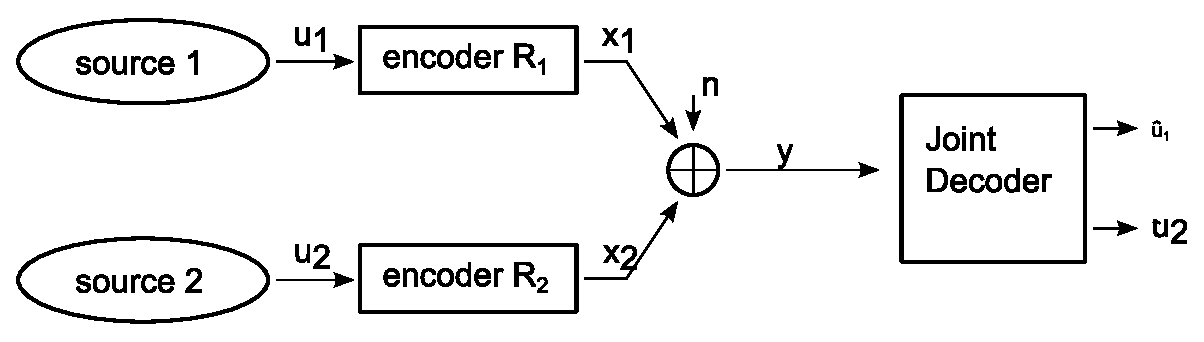
\includegraphics[scale=0.6]{Rate_Region_Example}
\end{figure}
\begin{itemize}
	\item How should we choose $R_1 $ and $R_2 $ to ensure error free decoding of \underline{both} signal streams?
	\item It is no longer sufficient to maximizie a single rate. Instead we have to consider rate pairs $(R_1, R_2)$
	\item All possible rate points, that allows error free decoding, define the rate region $\underline{C} $
	\item Possible desing goals of the system:
	\begin{itemize}
		\item maximized sumrate $R_{\text{sum}} = \underset{(R_1, R_2) \in \underline{C}}{\text{max}} R_1 + R_2 $ 
		\item maximize minimum user rate: $R_{\text{max-min}} = \underset{(R_1, R_2) \in \underline{C}}{\text{max}} \, \underset{i \in \{1, 2\}}{\text{min}} R_i $ 
	\end{itemize}
	\item Rate Region of two user Gaussian MAC \quad\textit{Anmerkung: Einschr\"ankungen}
	\begin{align}
		R_1 &< \log_2\bigl(1 + \frac{\mathcal{E}_1}{\sigma_n^2}\bigr) \label{eq:Formel_1}\\ 
		R_2 &< \log_2\bigl(1 + \frac{\mathcal{E}_2}{\sigma_n^2}\bigr)\label{eq:Formel_2} \\ 
		R_1 + R_2 &< \log_2\bigl(1 + \frac{\mathcal{E}_1 + \mathcal{E}_2}{\sigma_n^2}\bigr) 	\label{eq:Formel_3}	
	\end{align}
	\item Interpretation:
	\begin{itemize}
		\item \eqref{eq:Formel_1} and \eqref{eq:Formel_2}  (= single\,-to\,user constraint) are the ``single\,-\,user bounds´´, i.e., the maximum rates of user 1 and 2, if the other user was not there
		\item \eqref{eq:Formel_3} can be interpreted as the maximum rate if streams of users 1 and 2 were jointly encoded. The separate encoding in the MAC cannot yield a better performance
		\item Graphical represantation: \\
		\begin{tikzpicture}
		\tikzstyle{every node} = [font = \small]
			\path[draw,->,>=stealth'](0,-0.3)--
				(0,3) node [left] {$\log_2(1+\frac{\mathcal{E}_2}{\mathcal{E}_1 + \sigma_n^2})$}--
				(0,4) node [left] {$\log_2(1+\frac{\mathcal{E}_2}{\sigma_n^2})$}--
				(0,2) node [right] {achievable rate}--		
				(0,6) node [left] {$R_2$};
			\path[draw,->,>=stealth'](-0.3,0)--
				(3,0) node [above] {$\log_2(1+\frac{\mathcal{E}_1}{\mathcal{E}_2 + \sigma_n^2})$}--
				(4,0) node [below] {$\log_2(1+\frac{\mathcal{E}_1}{\sigma_n^2})$}--
				(6,0) node [below] {$R_1$};
			\path[draw](4,0)--
				(4,0.2) node [right] {D}--
				(4,2.8) node [left] {C}--
				(4,3) node {};
			\path[draw,dashed](3,0)--
				(3,4) node [above] {B};
			\path[draw](0,4)--
				(0.2,4) node [above] {A}--
				(3,4) node {};
			\path[draw,dashed](0,3)--
				(4,3) node {};
			\path[draw](3,4)--
				(4,3) node [above] {dominant face};
			\path[draw,dashed](1,6)--
				(6,1) node [above] {$R_1 + R_2 = \log_2(1 + \frac{\mathcal{E}_1 + \mathcal{E}_2}{\sigma_n^2}) $};
		\end{tikzpicture}
	\end{itemize}
	
	\item Observations:
	\begin{itemize}
		\item A\,-\,B is defined by \eqref{eq:Formel_2}
		\item C\,-\,D is defined by \eqref{eq:Formel_1}
		\item B\,-\,C is defined by \eqref{eq:Formel_3}
		\item A\,-\,B suggests that even if user 2 transmits with the same max. rate as in the single user case, user 1 can transmit with non-zero rate! $\rightarrow $ Multiuser communication enables ``free´´ rate gains!
		\item Which point on A\,-\,B\,-\,C,-\,D we choose, depends on the design criterion 	
	\end{itemize}		
	\item How do we achieve points on 	A\,-\,B\,-\,C,-\,D? 
	\begin{itemize}
		\item Both user use Gaussian codebooks
		\item B: 
		\begin{itemize}
			\item signal of user 1, $x_1$, is decoded first and $x_2 $ is treated as noise:
			\begin{align*}
				y &= x_1 + \underbrace{x_2 + n}_{\text{treat as noise}}\\ \rightarrow R_1 &< \log_2\bigl(1 + \frac{\mathcal{E}_1}{\mathcal{E}_2 + \sigma_n^2}\bigr)
			\end{align*}
			\item once $x_1 $ is known, we form 
			\begin{align*}
				y -x_1 &= x_2 + n\\ \rightarrow R_2 &< \log_2\bigl(1 + \frac{\mathcal{E}_s}{\sigma_n^2}\bigr)
			\end{align*}
			\item this approach is referred to as successive interference cancellation (SIC) and is a direct result of the chain rule in information theory:\\ $I(X_1, X_2, Y) = I(X_1, Y) + I(X_2; Y|X_1) $
		\end{itemize}
		\item C: same as B, but $X_1 $ and $X_2 $ change rules
		\item Points on A\,-\,B, C\,-\,D can be achieved by decreasing the rate of users 1 and 2 respectively (not desirable)
		\item Points on B\,-\,C (dominant face): Achievable by ``time-sharing´´, i.e., $\theta\cdot 100\% $ of the time we decode user 1 first and $(1 - \theta)100\% $ of the time we decode user 2 first, $ 0\leq \theta \leq 1 $ 
		\begin{align*}
			R_1 &< \theta\log_2\bigl(1 + \frac{\mathcal{E}_1}{\mathcal{E}_2 + \sigma_n^2}\bigr) + \bigl(1-\theta\bigr)\log_2\bigl(1 + \frac{\mathcal{E}_1}{\sigma_n^2}\bigr)\\
			R_2 &< \theta\log_2\bigl(1 + \frac{\mathcal{E}_2}{\sigma_n^2}\bigr) + \bigl(1-\theta\bigr)\log_2\bigl(1 + \frac{\mathcal{E}_2}{\mathcal{E}_1 + \sigma_n^2}\bigr)\\
			\rightarrow R_1 + R_2 &< \theta\Bigl(\log_2\bigl( 1 + \frac{\mathcal{E}_1}{\mathcal{E}_2 + \sigma_n^2}\bigr) + \log_2\bigl(1 + \frac{\mathcal{E}_2}{\sigma_n^2}\bigr)\Bigr) + \\ &+ \bigl( 1- \theta\bigr) \Bigl(\log_2\bigl(1 + \frac{\mathcal{E}_1}{\sigma_n^2}\bigr) + \log_2\bigl(1 + \frac{\mathcal{E}_2}{\mathcal{E}_1 + \sigma_n^2}\bigr)\Bigr) = \\ &= \theta\log_2\Bigl(\frac{\mathcal{E}_1 + \mathcal{E}_2 + \sigma_n^2}{\mathcal{E}_2 + \sigma_n^2}\cdot\frac{\mathcal{E}_2 + \sigma_n^2}{\sigma_n^2}\Bigr) \cdot\bigl(1 - \theta\bigr)\log_2\Bigl(\frac{\mathcal{E}_1 + \sigma_n^2}{\sigma_n^2} \cdot\frac{\mathcal{E}_1 + \mathcal{E}_2 + \sigma_n^2}{\mathcal{E}_1 + \sigma_n^2} = \\ &= \log_2\Bigl( 1 + \frac{\mathcal{E}_1 + \mathcal{E}_2}{\sigma_n^2}\Bigr)
		\end{align*}
	\end{itemize}
	\item Comparison with orthogonal transmission
	\begin{itemize}
		\item User 1 transmits for $\theta\cdot 100\% $ of the time and user 2 transmits for $(1-\theta)\cdot 100\%  $ of the time, $0\leq \theta\leq 1 $
		\item to keep average transmit power independent of $\theta$, the users transmit with powers $\frac{\mathcal{E}_1}{\theta} $ and $\frac{\mathcal{E}_2}{1 - \theta} $ 
		\item Rates: 
		\begin{align*}
			R_1 &< \theta\log_2\Bigl( 1 + \frac{\mathcal{E}_1}{\theta\sigma_n^2}\Bigr)\\
			R_2 &< \bigl(1 - \theta\bigr)\log_2\Bigl( 1 + \frac{\mathcal{E}_2}{(1 - \theta)\sigma_n^2}\Bigr)
		\end{align*}
		\item[] multiuser:\\
			\begin{tikzpicture}
				\path[draw,<->,>=stealth'] node[left] {}(0,5)  -- node[sloped, above] {$\mathcal{E}_1$} (10,5) node[right]{ user 1};
				\path[draw,<->,>=stealth'] (0,4)  -- node[sloped, above] {$\mathcal{E}_2$} (10,4) node[right]{ user 2};
			\end{tikzpicture}
		\item[] orthogonal:\\
			\begin{tikzpicture}
				\path[draw,<->,>=stealth']node[left] {} (0,3)  -- node[sloped, above] {$\frac{\mathcal{E}_1}{\theta}$}(4,3) ;
				\path[draw,<->,>=stealth']node{}(4,3) --node[sloped,above]{non-transmission period: $1 -\theta$}(10,3) node[right]{ user 1} ;
				\path[draw,<->,>=stealth']node{}(0,2)--node[sloped,above]{non-transmission period: $\theta$}(4,2);
				\path[draw,<->,>=stealth'] (4,2)  -- node[sloped, above] {$\frac{\mathcal{E}_2}{1 - \theta}$} (10,2)  node[right]{ user 2};
			\end{tikzpicture}
			\item sumrate:
			\begin{align*}
				R_1 + R_2 < \theta\log_2\Bigl(1 + \frac{\mathcal{E}_1}{\theta\sigma_n^2}\Bigr) + \bigl(1-\theta\bigr)\log_2\Bigl(1 + \frac{\mathcal{E}_2}{(1-\theta)\sigma_n^2}\Bigr) = R_{\text{sum}} 
			\end{align*}			
			\item Which $\theta $ maximizes sumrate?
			\begin{align*}
				\frac{\delta R_{\text{sum}}}{\delta\theta} \overset{!}{=}  0 \text{ leads to } \theta_{\text{opt}} = \frac{\mathcal{E}_1}{\mathcal{E}_1 + \mathcal{E}_2}	
			\end{align*}			 
			\item Maximum sumrate
			\begin{align*}
				R_{\text{sum}} &= \frac{\mathcal{E}_1}{\mathcal{E}_1 + \mathcal{E}_2}\log_2\Bigl(1 + \frac{\mathcal{E}_1 + \mathcal{E}_2}{\sigma_n^2}\Bigr) + \frac{\mathcal{E}_2}{\mathcal{E}_1 + \mathcal{E}_2}\log_2\Bigl(1 + \frac{\mathcal{E}_1 + \mathcal{E}_2}{\sigma_n^2}\Bigr) = \\ &= \log_2\Bigl(1 + \frac{\mathcal{E}_1 + \mathcal{E}_2}{\sigma_n^2}\Bigr)\\
				&\rightarrow \text{ same value as for general non-orthogonal transmission!}
			\end{align*}
			\item \underline{But:} In general, orthogonal transmission is suboptimal!\\
			\begin{tikzpicture}
			\tikzstyle{every node} = [font = \small]
				\path[draw,->,>=stealth'] (0,-0.3)--
					(0,4) node [left] {$R_2$};
				\path[draw,->,>=stealth'] (-0.3,0)--
					(5,0) node [below] {$R_1$};
				\path[draw] (0, 3)--
					(2,3) node {} --
					(4,2) node {}--
					(4,1.5) node [right] {non-orthogonal}--
					(4,0) node {};			
				\path[draw,dashed] (0,3) --
					(1.5,11/4) node[below] {orthogonal}--
					(3,2.5) node {}--
					(4,0) node{};
				\node[right] at (3,2.5) {optimal $\theta = \theta_{\text{opt}}$};
					\pgfsetplotmarksize{0.3ex}
					\pgfplothandlermark{\pgfuseplotmark{*}}
					\pgfplotstreamstart
					\pgfplotstreampoint{\pgfpoint{3cm}{2.5cm}}
					\pgfplotstreamend	
			\end{tikzpicture}	
	\end{itemize}
	\item 3 users case:
	\begin{align*}
		R_1 &< \log_2\Bigl(1 + \frac{\mathcal{E}_1}{\sigma_n^2}\Bigr)\\
		R_2 &< \log_2\Bigl(1 + \frac{\mathcal{E}_2}{\sigma_n^2}\Bigr)\\
		R_3 &< \log_2\Bigl(1 + \frac{\mathcal{E}_3}{\sigma_n^2}\Bigr)\\
		R_i + R_j &< \log_2\Bigl(1 + \frac{\mathcal{E}_i + \mathcal{E}_j}{\sigma_n^2}\Bigr),\quad i\neq j\\
		R_1 + R_2 + R_3 &< \log_2\Bigl(1 + \frac{\mathcal{E}_1 + \mathcal{E}_2 + \mathcal{E}_3}{\sigma_n^2}\Bigr)\\
		&\rightarrow \text{rate region } \mathbf{\mathcal{C}} \text{ has } 3! = 6 \text{ corner points}
	\end{align*}
	\item general case of K users
	\begin{itemize}
		\item define all non-empty subsets of $\mathbf{K} = \bigl\{1,\ldots, K\bigr\} $ as $ \mathbf{S} \in \mathbf{K}$,\\  e.g. $K = 2$: $\mathbf{K} = \bigl\{1, 2\bigr\}, \mathbf{S} = \bigl\{\{1\}, \{2\}, \{1, 2\}\bigr\} $ 
	\end{itemize}
	\item rate region $\mathbf{\mathcal{C}} $  is defined by
	\begin{align*}
		\sum_{k \in \mathbf{S}}R_k < \log_2\Bigl(1 + \frac{\sum_{k\in\mathbf{S}\mathcal{E}_k}}{\sigma_n^2}\Bigr)\quad\forall\, \mathbf{S}
	\end{align*}
	\item[$\rightarrow$] $\mathbf{\mathcal{C}} $  has $ K! $ corner points which can all be achieved by successive interference cancellation (SIC) 
\end{itemize}
\paragraph{Rate region for MIMO Users and Receivers}
\begin{itemize}
	\item Channel Model: $ \mathbf{y} = \sum_{k = 1}^{K}\mathbf{H}_k\mathbf{x}_k + \mathbf{n} $, with:
	\begin{itemize}
		\item User k has $N_{T,k} $ transmit antennas
		\item $N_R $ receive antennas
		\item $\mathbf{n} $: AWGN vector $\mathcal{N}(\mathbf{0},\sigma_n^2\mathbf{I})$
	\end{itemize}
	\item 2 Users case: 
	\begin{equation}
		\mathbf{y} = \mathbf{H}_1\mathbf{x}_1 + \mathbf{H}_2\mathbf{x}_2 + \mathbf{n}  \label{eq:Formel_7}
	\end{equation}	 
	\begin{itemize}
		\item Covariance matrix of the TX signal of user k: $\mathbf{Q}_k = \mathcal{E}\{\mathbf{x}_k\mathbf{x}_k^H\} $
		\item transmit power: $\mathcal{E}_k = \text{tr}\{\mathbf{Q}_k\} $
	\end{itemize}
	\item rate region for 2 user case and given $\mathbf{Q}_k$
	\begin{itemize}
		\item $\mathbf{Q}_k $ given, for example 
		\begin{itemize}
			\item[a)] $\mathbf{Q}_k$ optimal for single user case $\rightarrow \mathbf{Q}_k = \mathbf{U}_k\mathbf{\Lambda}_k\mathbf{U}_k^H $, where:
			\begin{itemize}
				\item $\mathbf{U}_k $ is an unitary matrix 
				\item obtained from $\mathbf{H}_k = \mathbf{U}_k\mathbf{\Sigma}_k\mathbf{V}_k^H $
				\item $\mathbf{\Lambda}_k = \text{diag}\{\mathcal{E}_{k,1},\mathcal{E}_{k,2},\ldots,\mathcal{E}_{k,N_T}\} $ with $\mathcal{E}_{l,i} $ obtained from waterfilling and $\sum_{i = 1}^{N_{Tk}}\mathcal{E}_{k,i} = \mathcal{E}_k $
			\end{itemize}
			\item[b)] $\mathbf{Q}_k = \frac{\mathcal{E}_k}{N_{T,k}}\mathbf{I}_{N_{T,k}} $ if $\mathbf{H}_k $ is not known at transmitter
		\end{itemize}
		\item for given $\mathbf{Q}_1 $ and $\mathbf{Q}_2 $ we can obtain the rate region as direct extension of the SISO case
		\begin{align}
			R_1 &< \log_2\bigl|\mathbf{I} + \frac{1}{\sigma_n^2}\mathbf{H}_1\mathbf{Q}_1\mathbf{H}_1^H\bigr|\label{eq:Formel_4}\\
			R_2 &< \log_2\bigl|\mathbf{I} + \frac{1}{\sigma_n^2}\mathbf{H}_2\mathbf{Q}_2\mathbf{H}_2^H\bigr|\label{eq:Formel_5}\\
			R_1 + R_2 &< \log_2\bigl|\mathbf{I} + \frac{1}{\sigma_n^2}\sum_{i = 1}^{2}\mathbf{H}_i\mathbf{Q}_i\mathbf{H}_i^H\bigr|\label{eq:Formel_6}			
		\end{align}
		\begin{itemize}
			\item equation \ref{eq:Formel_4} and equation  \ref{eq:Formel_5} are the single user bounds,
			\item equation \ref{eq:Formel_6} is the bound for the joint encoding of both users
		\end{itemize}
		\item graphical represantation\\
		\begin{tikzpicture}
			\tikzstyle{every node} = [font = \small]
				\path[draw,->,>=stealth'] (0,-0.3)--
					(0,4) node [left] {$R_2$};
				\path[draw,->,>=stealth'] (-0.3,0)--
					(5,0) node [above] {$R_1$};
				\path[draw] (-0.1, 3)--
					(0,3) node[left]{$\log_2|\mathbf{I} + \frac{1}{\sigma_n^2}\mathbf{H}_2 \mathbf{Q}_2\mathbf{H}_2^H|$}--
					(0.3,3) node[above] {A}--
					(2,3) node[above] {B} --
					(3,2.5) node[right]{$R_1 + R_2$}--
					(4,2) node[right] {C}--
					(4,0.3) node [right] {D}--
					(4,-0.1) node[below] {$\log_2|\mathbf{I} + \frac{1}{\sigma_n^2}\mathbf{H}_1 \mathbf{Q}_1\mathbf{H}_1^H|$};		
		\end{tikzpicture}
	\item Points on A\,-\,B\,-\,C\,-\,D can be achieved in a similar manner as for SISO case	
	\item e.g. bound C can be achieved by SIC
	\item At B we have 
	\begin{align*}
		R_2 &= \log_2\bigl|\mathbf{I} + \frac{1}{\sigma_n^2}\mathbf{H}_2\mathbf{Q}_2\mathbf{H}_2^H\bigr|\\
		R_1 &= \log_2\bigl|\mathbf{I} + \frac{1}{\sigma_n^2}\sum_{i = 1}^{2}\mathbf{H}_i\mathbf{Q}_i\mathbf{H}_i^H\bigr| - R_2\\
		\rightarrow &\text{ user 1 transmits with rate}\\
		R_1 &= \log_2\bigl|\mathbf{I} + \frac{1}{\sigma_n^2}(\mathbf{I} + \frac{1}{\sigma_n^2}\mathbf{H}_2\mathbf{Q}_2\mathbf{H}_2^H)^{-1}\mathbf{H}_1\mathbf{Q}_1\mathbf{H}_1^H\bigr|
	\end{align*}
	\item How to achieve rates at B? $\rightarrow $ Treat $\mathbf{H}_2\mathbf{x}_2 + \mathbf{n} $ in equation  \ref{eq:Formel_7} as noise with covariance matrix $ \mathbf{Q}_N = \mathbf{H}_2\mathbf{Q}_2\mathbf{H}_2^H + \sigma_n^2\mathbf{I} $
	\item[$\rightarrow$] equivalent channel matrix with white noise: $\mathbf{r} = \mathbf{Q}_N^{-\frac{1}{2}}\mathbf{y} = 	\mathbf{Q}_N^{-\frac{1}{2}}\mathbf{H}_1\mathbf{x}_1 + \tilde{\mathbf{n}} $ where $ \tilde{\mathbf{n}} $ is white noise with covariance $\mathbf{I}$. \\ \textit{Anmerkung: Rauschen war vorher farbig, muss ``gewei"st"\  werden.} 
	\begin{align*}
		\rightarrow R_1 &= \log_2\bigl|\mathbf{I} + \underbrace{\mathbf{Q}_N^{-\frac{1}{2}} \mathbf{H}_1}_{\mathbf{H}}\mathbf{Q}_1\underbrace{\mathbf{H}_1^H\mathbf{Q}_N^{-\frac{1}{2}}}_{\mathbf{H_{eq}^H}}\bigr|  = \log_2\Bigl(\bigl|\mathbf{Q}_N^{\frac{1}{2}} + \mathbf{Q}_N^{-\frac{1}{2}}\mathbf{H}_1\mathbf{Q}_1\mathbf{H}_1^H\bigr|\cdot\bigl|\mathbf{Q}_N^{-\frac{1}{2}}\bigr|\Bigr)\\
		&= \log_2\bigl|\mathbf{I} + \mathbf{Q}_N^{-1}\mathbf{H}_1\mathbf{Q}_1\mathbf{H}_1^H\bigr| = \\
		&= \log_2\bigl|\mathbf{I} + \frac{1}{\sigma_n^2}\bigl(\mathbf{I} + \frac{1}{\sigma_n^2}\mathbf{H}_2\mathbf{Q}_2\mathbf{H}_2^H\bigr)^{-1}\mathbf{H}_1\mathbf{Q}_1\mathbf{H}_1^H\bigr|
	\end{align*}
	\item[$\rightarrow$] we can achieve $R_1 $ in B by treating user 2 as noise
	\item[$\rightarrow$] once user 1 is detected, we can subtract its contribution from the received signal and detect user 2
	\begin{itemize}
		\item[$\Rightarrow$] user 2 can transmit with maximum single user rate
	\end{itemize}
	\item[$\rightarrow$] bound C can be achieved by SIC similar to SISO case
	\item points on B\,-\,C are achieved through time sharing
	\end{itemize}
	\item extension to K user case $\rightarrow $ analogous to SISO case
	\item Note: Different choices for $Q_k $ will lead to different rate regions
	\item Example: $ K = 2$
	\begin{tikzpicture}
		\tikzstyle{every node} = [font = \small]
				\path[draw,->,>=stealth'] (0,-0.3)--
					(0,5) node [left] {$R_2$};
				\path[draw,->,>=stealth'] (-0.3,0)--
					(7,0) node [below] {$R_1$};
				\path[draw] (0, 4)--
					(1.5,4) node[above] {$\mathbf{Q}_1^a, \mathbf{Q}_2^a$}--
					(3,4) node{}--
					(5,2) node{}--
					(5,0) node{};
				\path[draw,dashed](0,3)--
					(4.5,3) node[right]{$\mathbf{Q}_1^b, \mathbf{Q}_2^b$}--
					(6.5,1.5) node {}--
					(6.5,0) node{};
	\end{tikzpicture}
	\item[$\rightarrow$] $\mathbf{Q}_1 $ and $ \mathbf{Q}_2 $ can be optimized to achieve desired trade-off between  performance of users 1 and 2
\end{itemize}
\subsection{Broadcast Channel}
We consider:
\begin{itemize}
	\item uplink\,-\,downlink duality
	\item rate region
\end{itemize}
\subsubsection{Multiplexing Gain\,-\,Degrees of freedom}
\paragraph{Downlink scenarios:}
\begin{itemize}
	\item $N_R $ antennas at transmitter, single antennas at the users
	\item user k receives: $ \mathbf{y}_k = \mathbf{h}_k^H\mathbf{x} + \mathbf{n}_k $, with:
	\begin{itemize}
		\item $N_R $ dimensional channel vector of user k: $\mathbf{h}_k^H $
		\item $n_k$: AWGN at user k
		\item $\mathbf{x} $ transmit vector  
	\begin{figure}[ht]
		\centering
		\psfrag{sender}[bl][bl][3]{$\underline{\text{x}}$}
		\psfrag{CH1}[br][br]{$h_1^H$}
		\psfrag{CH2}[br][br]{$h_2^H$}
		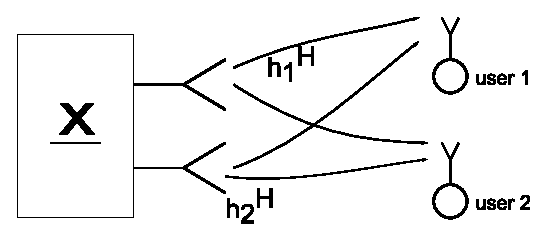
\includegraphics[scale=0.8]{BroadcastChannel_scenario.eps}
	\end{figure}
	\end{itemize}
	\item How many independent signal streams can we transmit?
	\begin{itemize}
		\item Consider transmit signal: $\mathbf{x} = \sum\limits_{k = 1}^{K}\mathbf{h}_k\mathbf{x}_k $, with TX transmit vector $\mathbf{n}_k $ and symbol $x_k $ is intended for user k
	\end{itemize}
	\item received signal of user k: $y_k = \sum\limits_{k = 1}^{K}(\mathbf{h}_k^H\mathbf{n}_i)\mathbf{x}_i + n_k $
	\item if all $\mathbf{h}_k $ were orthogonal and we chose $\mathbf{n}_k = \mathbf{h}_k $, the received signal would be: \\ $y_k = ||h_k||^2\mathbf{x}_k + n_k $
	\item if $N_R \geq K$, we can transmit simultaneously and interference free to all K users\\ $\Rightarrow $ multiplexing gain $= \text{min}\{K,N_k\} $
\item In practice, the $\mathbf{h}_k $ will not be orthogonal
\begin{itemize}
	\item[$\rightarrow$] choose $\mathbf{n}_k $ such that it lies in the null space of $\begin{bmatrix}
	\mathbf{h}_1 & \ldots & \mathbf{h}_{k-1} & \mathbf{h}_{k+1} & \ldots & \mathbf{h}_K \end{bmatrix}	 $
	\item[$\rightarrow$] always possible if $ \mathbf{h}_1,\ldots, \mathbf{h}_K $ are linearly independent
	\item[$\rightarrow$] multiplexing gain ( $= $ degrees of freedom) is equal to $ \text{min}\{K, N_R\} $
\end{itemize}
\item we can transmit interference free to $K\leq N_R $ users \\ \quad \textit{Anmerkung: Falls TX viele Antennen, aber RX nur eine hat $\Rightarrow $ begrenzter Nutzen: SNR Verbesserung, kein Multiplexing Gain; falls TX viele Antennen und viele RX vorhanden sind $\Rightarrow $ RX erscheinen als Antennenarray $\rightarrow $ hoher Multiplexing Gain}
\end{itemize}

\subsubsection{Uplink\,-\,Downlink  Duality}
\begin{itemize}
	\item How should we choose signature vectors to achieve a certain SNR at users?
	\item Difficult problem since optimal (in the SINR sense) $\mathbf{u}_k $ are not orthogonal $\rightarrow $ signature of user $k$, $\mathbf{u}_k $, influences SINR at all other users!
	\item On the other hand, the uplink problem was much easier to solve, since the receive filter of user $k$, $\mathbf{f}_k$, was not affected by receive filters of other users! (vgl. Point\,-\,to\,-\,Point $\rightarrow $ detection problem
	\item[$\Rightarrow$] We establish a duality between the uplink and downlink, that allows us to solve the more challenging downlink problem by solving an equivalent uplink problem.
\end{itemize}
\paragraph{Downlink:}
\begin{itemize}
	\item transmit signal
	\begin{align*}
		\mathbf{x}_{dl} = \sum\limits_{k = 1}^{K}\mathbf{u}_kx_{dl,k}
	\end{align*}
	\item received signal at user $k$
	\begin{align*}
		y_{dl,k} = \mathbf{h}_k^H\mathbf{u}_kx_{dl,k} + \sum\limits_{j \neq k}\mathbf{h}_k^H\mathbf{u}_jx_{dl,j} + u_{dl,k}
	\end{align*}
	\item SINR of user $k$
	\begin{align*}
		\text{SINR}_k^{dl} = \frac{\mathcal{E}_{dl,k}|\mathbf{u}_k^H\mathbf{h}_k|^2}{\sigma_n^2 + \sum\limits_{j \neq k}\mathcal{E}_{dl,j}|\mathbf{h}_j^H\mathbf{h}_k|^2},\quad 1\leq k \leq K
	\end{align*}
	\item where: $\mathcal{E}_{dl,k} = \mathcal{E}\bigl\{|x_{dl,k}|^2 \bigr\}; \quad \sigma_n^2 = \mathcal{E}\bigl\{|n_{dl,k}|^2\bigr\} $
	\item Using: 
	\begin{align*}
		a_k = \frac{\text{SINR}_k^{dl}}{(1 + \text{SINR}_k^{dl})|\mathbf{h}_k^H\mathbf{u}K|^2}
	\end{align*}
	we can rewrite the the SINR expressions as:
	\begin{align*}
		\boxed{\bigl(\mathbf{I}_K - \text{diag}\{a_1, \ldots, a_k\}\mathbf{A}\bigr)\mathbf{p}_{dl} = \sigma_n^2\mathbf{a}}
	\end{align*}
	where:
	\begin{align*}
		\mathbf{a} &= \begin{bmatrix} a_1,\ldots,a_k\end{bmatrix}^T \\
		\mathbf{A} &= 
		\begin{bmatrix}
			|u_1^Hh_1|^2 & |u_2^Hh_1|^2 & \ldots & |u_K^Hh_1|^2	\\
			\vdots \\
			|u_1^Hh_K|^2 & \ldots & & |u_K^Hh_K|^2		
		\end{bmatrix} \\
		\mathbf{p}_{dl} &= 
		\begin{bmatrix}
			\mathcal{E}_{dl,1},\ldots, \mathcal{E}_{dl,K}	
		\end{bmatrix}^T
	\end{align*}
	\item[$\rightarrow$] We can easily calculate transmit powers $\mathcal{E}_{dl,k} $ required to achieve desired $\text{SINR}_k^{dl}, 1\leq k_1\leq K, $ for given signature (precoding) vectores $u_k, 1\leq k\leq K $ 
	\item Block diagramm: 
	\begin{figure}[ht]
		\centering	
		\psfrag{Eingang1}[bl][bl][1]{$x_{dl,1} $}
		\psfrag{Eingang2}[bl][bl][1]{$x_{dl,K} $}
		\psfrag{Nutzer1}[bl][bl][1]{$\mathbf{u}_1 $}
		\psfrag{Nutzer2}[bl][bl][1]{$\mathbf{u}_2 $}
		\psfrag{Kanalmatrix}[bl][bl][1]{$\mathbf{H}^* $}
		\psfrag{Rauschen1}[bl][bl][1]{$n_{dl,1} $}
		\psfrag{Rauschen2}[bl][bl][1]{$n_{dl,k} $}
		\psfrag{Ausgang1}[bl][bl][1]{$y_{dl,1} $}
		\psfrag{Ausgang2}[bl][bl][1]{$y_{dl,K} $}
		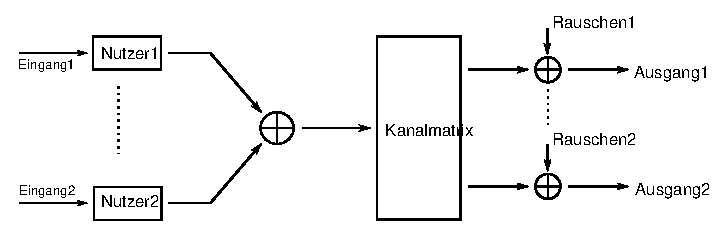
\includegraphics[scale=0.8]{Downlink_MIMO}		
	\end{figure}
\end{itemize}
\paragraph{Uplink:} 
Use downlink signatures, $\mathbf{h}_k$, as receive filters, $\mathbf{f}_k$
\begin{itemize}
	\item block diagramm: 
	\begin{figure}[ht]
		\centering	
		\psfrag{Eingang1}[bl][bl][1]{$x_{ul,1} $}
		\psfrag{Eingang2}[bl][bl][1]{$x_{ul,K} $}
		\psfrag{Nutzer1}[bl][bl][1]{$\mathbf{u}_1 $}
		\psfrag{Nutzer2}[bl][bl][1]{$\mathbf{u}_2 $}
		\psfrag{Kanalmatrix}[bl][bl][1]{$\mathbf{H}^* $}
		\psfrag{Rauschen1}[bl][bl][1]{$n_{ul} $}
		\psfrag{Ausgang1}[bl][bl][1]{$y_{ul,1} $}
		\psfrag{Ausgang2}[bl][bl][1]{$y_{ul,K} $}
		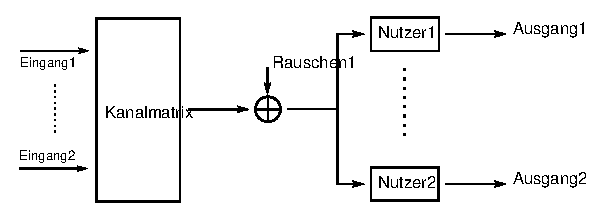
\includegraphics[scale=0.8]{Uplink_MIMO}		
	\end{figure}
	\item Signal model:
	\begin{align*}
		y_{ul,k} &= \mathbf{u}_k^H\bigl(\mathbf{Hx}_{ul} + \mathbf{u}_{ul}\bigr) 
	\end{align*}	
		with 
	\begin{align*}
		\mathbf{H} &= 
		\begin{bmatrix}
			\mathbf{h}_1 & \ldots & \mathbf{h}_K
		\end{bmatrix} ,\quad \mathbf{x}_{ul} = 
		\begin{bmatrix}
			x_{ul,1} & \ldots & x_{ul,K}
		\end{bmatrix}^T , \quad \mathbf{u}_{ul} = 
		\begin{bmatrix}
			u_{ul,1} & \ldots & u_{ul,K}
		\end{bmatrix}^T 
	\end{align*}		
	\begin{align}
		\rightarrow y_{ul,k} &= \mathbf{u}_k^H\mathbf{h}_kx_{ul,k} + \sum\limits_{j \neq k}\mathbf{u}_k\mathbf{h}_jx_{ul,j} + \mathbf{n}_k^H\mathbf{u}_{ul}\\
		\rightarrow \text{SINR}_k^{ul} &= \frac{\mathcal{E}_{ul,k}|\mathbf{u}^H\mathbf{h}_k|^2}{\sigma_n^2 + \sum\limits_{j\neq k}\mathcal{E}_{ul,j}|\mathbf{u}_k^H\mathbf{h}_j|^2}\label{eq:Formel_8}
	\end{align}
	where we used $\mathbf{u}_k^H\mathbf{u}_k = 1 $ and $ \mathcal{E}_{ul,K} = \mathcal{E}\bigl\{|x_{ul,K}|^2\bigr\} $ 
	\item we define: $ b_k = \frac{\text{SINR}_k^{ul}}{(1 + \text{SINR}_k^{ul})|\mathbf{u}_k^H\mathbf{h}_k|^2} $
	\item we can rewrite SINR epression \eqref{eq:Formel_8} as : 
	\begin{align*}
		\sigma_n^2 + \sum\limits_{j\neq k}\mathcal{E}_{ul,j}\bigl|\mathbf{u}_k^H\mathbf{h}_j\bigr|^2 = \frac{1}{\text{SINR}_k^{ul}} \mathcal{E}_{ul,k}\bigl|\mathbf{u}_k^H\mathbf{h}_k\bigr|^2
	\end{align*}
	\begin{align*}
		\underbrace{\bigl(1 + \frac{1}{\text{SINR}_k^{ul}}\bigr)\bigl|\mathbf{u}_k^H\mathbf{h}_k\bigr|^2}_{\frac{1}{b_k}}\mathcal{E}_{ul,k} - \sum\limits_{j = 1}^{K}\mathcal{E}_{ul,k}\bigl|\mathbf{u}_k^H\mathbf{h}_k\bigr|^2 = \sigma_n^2
	\end{align*}
	\begin{align*}
		\rightarrow \mathcal{E}_{ul,k} - b_k\sum\limits_{j = 1}^{K}\mathcal{E}_{ul,j}\bigl|\mathbf{u}_k^H\mathbf{h}_j\bigr|^2 = b_k\sigma_n^2
	\end{align*}
	\item matrix notation:
	\begin{align*}
		\begin{bmatrix}
			\mathbf{I}_K - \text{diag}\bigl\{b_1,\ldots, b_K\bigr\}\mathbf{A}^T\mathbf{p}_{ul} = \sigma_n^2\cdot \mathbf{b}
		\end{bmatrix}
	\end{align*}
	\item where: $\mathbf{A} $ was defined for downlink case
	\begin{align*}
		\mathbf{p}_{ul} &= \begin{bmatrix} \mathcal{E}_{ul,1} & \ldots & \mathcal{E}_{ul,K}\end{bmatrix}^T \\
		\mathbf{b} &= \begin{bmatrix}b_1 & \ldots & b_K\end{bmatrix}^T				
	\end{align*}
	\item we can calculate power allocation vector $\mathbf{p}_{ul} $ for given $\text{SINR}_1^{ul} $ and $ \mathbf{u}_k,\quad 1\leq k \leq K $ 
\end{itemize} 
\paragraph{Comparison:} Assume, we want to achieve same SINR in uplink and downlink
\begin{itemize}
	\item[$\rightarrow$] $\text{SINR}_k^{ul}  = \text{SINR}_k^{dl} \quad \forall\quad k $ or equivalently $ a_k = b_k,\quad \forall\quad k $ !
	\item[] What sum power do we need in both uses?
	\begin{align*}
		\mathbf{p}_{dl} &= \sigma_n^2\bigl(\mathbf{I} - \text{diag}\{a_1, \ldots, a_K\}\mathbf{A}\bigr)^{-1}\mathbf{a} = \\
		&= \sigma_n^2\bigl(\mathbf{D}_a - \mathbf{A}\bigr)^{-1}\cdot\mathbf{1}
	\end{align*}
	where: $\mathbf{D}_a = \text{diag}\{\frac{1}{a_1}, \ldots, \frac{1}{a_K}\} $ and $ \mathbf{1} = \begin{bmatrix}	1 & 1 & 1 & \ldots & 1 \end{bmatrix}^T $ 
	\begin{align*}
		\mathbf{p}_{ul} = \sigma_n^2(\mathbf{D}_b - \mathbf{A}^T)^{-1}\cdot \mathbf{1}
	\end{align*}
	where: $\mathbf{D}_b = \text{diag}\{\frac{1}{b_1}, \ldots ,\frac{1}{b_K}\} $
	\begin{align*}
		\sum\limits_{k = 1}^{K}\mathcal{E}_{dl,k} &= \mathbf{1}^T\mathbf{p}_{dl} = \sigma_n^2\mathbf{1}^T\bigl(\mathbf{D}_a - \mathbf{A}\bigr)^{-1}\cdot\mathbf{1}\\
		&= \sigma_n^2\mathbf{1}^T\bigl(\mathbf{D}_b - \mathbf{A}\bigr)^{-1}\mathbf{1} \\
		&= \sigma_n^2\bigl[\mathbf{1}^T\bigl(\mathbf{D}_b - \mathbf{A}\bigr)^{-1}\mathbf{1}\bigr]^T \\
		&= \sigma_n^2\mathbf{1}^T\bigl[\bigl(\mathbf{D}_b - \mathbf{A}\bigr)^{-1}\bigr]^T\mathbf{1} \\
		&= \sigma_n^2\mathbf{1}^T\bigl(\underbrace{\mathbf{D}_b^T}_{\mathbf{D}_b} - \mathbf{A}^T\bigr)^{-1}\\cdot\mathbf{1} = \sum\limits_{k = 1}^{K}\mathcal{E}_{ul,k}
	\end{align*}
\end{itemize}
\paragraph{Conclusions:}
\begin{itemize}
	\item We can achieve any desired $\text{SINR}_k^{dl},\forall\, k,$ in the downlink by using filters optimized for uplink transmission as signature (precoding) vectors and the same sum power as in the uplink
	\item suitable filters may be MMSE or ZF filters $ \mathbf{u}_k = \mathbf{f}_k, \quad \forall \, k $
	\item Note that, in general, $\mathcal{E}_{ul,k} \neq \mathcal{E}_{dl,k} $, only the sum powers are equal!
	\item[$\rightarrow$] \fbox{\parbox{\textwidth}{For linear precoding, we can solve the more challenging problem via solving an equivalent uplink problem!}}
\end{itemize}
\paragraph{Extension:} This concept can be extended to nonlinear receivers as well. In this case the DFE receiver in the uplink is dual to a nonlinear Tamlinson\,-\,Harashima (TH) precoder in the downlink.

\subsubsection{Rate Region (only SISO)}
\begin{itemize}
	\item two user case: $ y_k = h_kx + n_k\,,\quad k \in \{1,2\} $
	\item Capacity can be achieved with so\,-\,called \textit{Costa Cor (dirty paper)} precoding
	\item In this scheme, the signal of ine user is processed such that it does not impair the receiver of the other user, while the signal of the other user is treated as Gaussian noise at the receiver of the first user.
	\item[$\rightarrow$] Thus, the achievable rates would be
	\begin{align*}
		R_1 &< \log_2\bigl(1 + \frac{|h_1|^2\mathcal{E}_1}{\sigma_n^2}\bigr)\\
		R_2 &< \log_2\bigl(1 + \frac{|h_2|^2\mathcal{E}_2}{\sigma_n^2 + |h_1|^2\mathcal{E}_1}\bigr)			
	\end{align*}	 
	\item $\mathcal{E}_1 $ and $\mathcal{E}_2 $ can be optimized as they both occure at the same transmitter
\end{itemize}
\end{document}				